So far in this chapter, work-items have communicated with other workitems in the work-group by exchanging data through work-group local memory and by synchronizing via implicit or explicit barrier functions, depending on how the kernel is written.\par

In Chapter 4, we discussed another grouping of work-items. A subgroup is an implementation-defined subset of work-items in a work-group that execute together on the same hardware resources or with additional scheduling guarantees. Because the implementation decides how to group work-items into sub-groups, the work-items in a sub-group may be able to communicate or synchronize more efficiently than the work-items in an arbitrary work-group.\par

This section describes the building blocks for communication 
among work-items in a sub-group. Note that sub-groups are currently implemented only for ND-range kernels and sub-groups are not expressible through hierarchical kernels.\par

\hspace*{\fill} \par %插入空行
\textbf{Synchronization via Sub-Group Barriers}

Just like how the work-items in a work-group in an ND-range kernel may synchronize using a work-group barrier function, the work-items in a sub-group may synchronize using a sub-group barrier function. Whereas the work-items in a work-group synchronize by calling a group\_barrier function or the barrier function in the nd\_item class, the work-items in a sub-group synchronize by calling a group\_barrier function or the barrier function in a special sub\_group class that may be queried from the nd\_item class, as shown in Figure 9-11.\par

\hspace*{\fill} \par %插入空行
Figure 9-11. Querying and using the sub\_group class
\begin{lstlisting}[caption={}]
h.parallel_for(nd_range{{size}, {16}}, [=](nd_item<1> item) {
	auto sg = item.get_sub_group();
	...
	sg.barrier();
	...
});
\end{lstlisting}

Like the work-group barrier, the sub-group barrier may accept optional arguments to more precisely control the barrier operation. Regardless of whether the sub-group barrier function is synchronizing global memory or local memory, synchronizing only the work-items in the sub-group is likely cheaper than synchronizing all of the work-items in the work-group.\par

\hspace*{\fill} \par %插入空行
\textbf{Exchanging Data Within a Sub-Group}

Unlike work-groups, sub-groups do not have a dedicated memory space for exchanging data. Instead, work-items in the sub-group may exchange data through work-group local memory, through global memory, or more commonly by using sub-group collective functions.\par

As described previously, a collective function is a function that describes an operation performed by a group of work-items, not an individual work-item, and because a barrier synchronization function is an operation performed by a group of work-items, it is one example of a collective function.\par

Other collective functions express common communication patterns. We will describe the semantics for many collective functions in detail later in this chapter, but for now, we will briefly describe the broadcast collective function that we will use to implement matrix multiplication using sub-groups.\par

The broadcast collective function takes a value from one work-item in the group and communicates it to all other work-items in the group. An example is shown in Figure 9-12. Notice that the semantics of the broadcast function require that the local\_id identifying which value in the group to communicate must be the same for all work-items in the group, ensuring that the result of the broadcast function is also the same for all work-items in the group.\par

\hspace*{\fill} \par %插入空行
Figure 9-12. Processing by the broadcast function
\begin{center}
	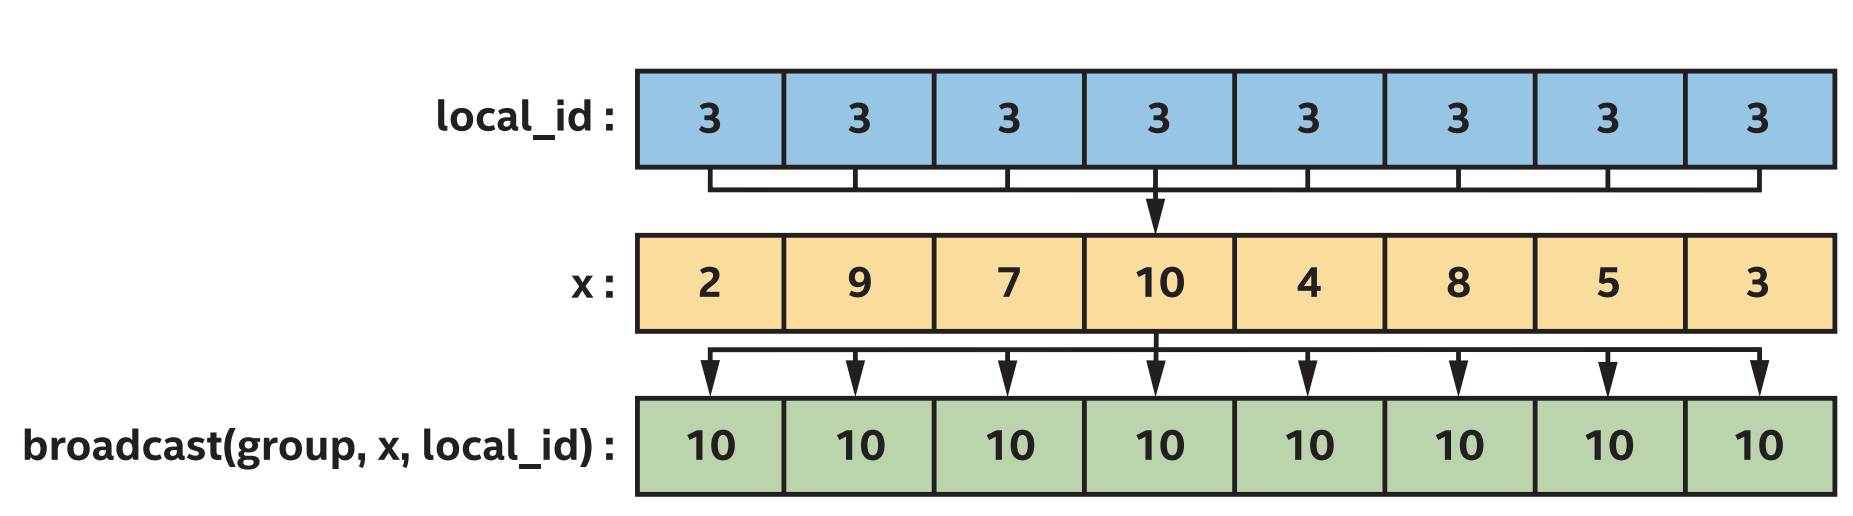
\includegraphics[width=1.\textwidth]{content/chapter-9/images/7}
\end{center}

If we look at the innermost loop of our local memory matrix multiplication kernel, shown in Figure 9-13, we can see that the access to the matrix tile is a broadcast, since each work-item in the group reads the same value out of the matrix tile.\par

\hspace*{\fill} \par %插入空行
Figure 9-13. Matrix multiplication kernel includes a broadcast operation
\begin{lstlisting}[caption={}]
h.parallel_for<class MatrixMultiplication>(
	nd_range<2>{ {M, N}, {1, tileSize} }, [=](nd_item<2> item) {
	...
	
	// Perform computation using the local memory tile, and
	// matrix B in global memory.
	for( size_t k = 0; k < tileSize; k++ ) {
		// Because the value of k is the same for all work-items
		// in the group, these reads from tileA are broadcast
		// operations.
		sum += tileA[k] * matrixB[kk + k][n];
	}
	...
});
\end{lstlisting}

We will use the sub-group broadcast function to implement a matrix multiplication kernel that does not require work-group local memory or barriers. On many devices, sub-group broadcasts are faster than broadcasting with work-group local memory and barriers.\par

\hspace*{\fill} \par %插入空行
\textbf{A Full Sub-Group ND-Range Kernel Example}

Figure 9-14 is a complete example that implements matrix multiplication using sub-groups. Notice that this kernel requires no work-group local memory or explicit synchronization and instead uses a sub-group broadcast collective function to communicate the contents of the matrix tile among work-items.\par

\hspace*{\fill} \par %插入空行
Figure 9-14. Tiled matrix multiplication kernel expressed with NDrange parallel\_for and sub-group collective functions
\begin{lstlisting}[caption={}]
// Note: This example assumes that the sub-group size is 
// greater than or equal to the tile size!
static const int tileSize = 4;

h.parallel_for(
nd_range<2>{{M, N}, {1, tileSize}}, [=](nd_item<2> item) {
	auto sg = item.get_sub_group();
	
	// Indices in the global index space:
	int m = item.get_global_id()[0];
	int n = item.get_global_id()[1];
	
	// Index in the local index space:
	int i = item.get_local_id()[1];
	
	T sum = 0;
	for (int_fast64_t kk = 0; kk < K; kk += tileSize) {
		// Load the matrix tile from matrix A.
		T tileA = matrixA[m][kk + i];
		
		// Perform computation by broadcasting from the matrix
		// tile and loading from matrix B in global memory. The loop
		// variable k describes which work-item in the sub-group to
		// broadcast data from.
		for (int k = 0; k < tileSize; k++)
			sum += intel::broadcast(sg, tileA, k) * matrixB[kk + k][n];
	}

	// Write the final result to global memory.
	matrixC[m][n] = sum;
});
});
\end{lstlisting}



































